\documentclass[aspectratio=169, 11pt]{beamer}

% ═══════════════════════════════════════
% THEME AND PACKAGES
% ═══════════════════════════════════════
\usetheme{Madrid}
\usecolortheme{seahorse}
\usepackage{graphicx}
\usepackage{amsmath}
\usepackage{booktabs}
\usepackage{tikz}
\usepackage{hyperref}
\usepackage{listings}
\usepackage{algorithm}
\usepackage{algorithmic}
\usepackage{multicol}
\usepackage{adjustbox}
\usetikzlibrary{shapes.geometric, arrows, positioning, fit, calc, backgrounds, decorations.markings}

% ═══════════════════════════════════════
% COLOR SCHEME
% ═══════════════════════════════════════
\definecolor{darkbg}{RGB}{13,13,26}
\definecolor{cardbg}{RGB}{26,26,46}
\definecolor{neongreen}{RGB}{0,255,136}
\definecolor{accentblue}{RGB}{51,153,255}
\definecolor{warnorange}{RGB}{255,153,51}
\definecolor{dangerred}{RGB}{255,51,51}
\definecolor{softgray}{RGB}{136,146,176}
\definecolor{darkblue}{RGB}{0,51,102}

\setbeamercolor{background canvas}{bg=darkbg}
\setbeamercolor{normal text}{fg=white}
\setbeamercolor{frametitle}{fg=neongreen, bg=cardbg}
\setbeamercolor{title}{fg=neongreen}
\setbeamercolor{subtitle}{fg=softgray}
\setbeamercolor{author}{fg=white}
\setbeamercolor{date}{fg=softgray}
\setbeamercolor{institute}{fg=softgray}
\setbeamercolor{item}{fg=neongreen}
\setbeamercolor{subitem}{fg=accentblue}
\setbeamercolor{block title}{bg=cardbg, fg=neongreen}
\setbeamercolor{block body}{bg=cardbg!70!darkbg, fg=white}
\setbeamercolor{block title alerted}{bg=dangerred!30, fg=dangerred}
\setbeamercolor{block body alerted}{bg=dangerred!10, fg=white}
\setbeamercolor{block title example}{bg=neongreen!20, fg=neongreen}
\setbeamercolor{block body example}{bg=neongreen!5!darkbg, fg=white}

\setbeamertemplate{navigation symbols}{}
\setbeamertemplate{footline}{
    \leavevmode\hbox{%
    \begin{beamercolorbox}[wd=.333333\paperwidth,ht=2.5ex,dp=1.25ex,center]{author in head/foot}%
        \usebeamerfont{author in head/foot}\textcolor{softgray}{\insertshortauthor}
    \end{beamercolorbox}%
    \begin{beamercolorbox}[wd=.333333\paperwidth,ht=2.5ex,dp=1.25ex,center]{title in head/foot}%
        \usebeamerfont{title in head/foot}\textcolor{neongreen}{\insertshorttitle}
    \end{beamercolorbox}%
    \begin{beamercolorbox}[wd=.333333\paperwidth,ht=2.5ex,dp=1.25ex,right]{date in head/foot}%
        \textcolor{softgray}{\insertframenumber{}/\inserttotalframenumber\hspace*{2ex}}
    \end{beamercolorbox}}%
}

\lstset{
  basicstyle=\ttfamily\tiny\color{white},
  frame=single,
  breaklines=true,
  backgroundcolor=\color{cardbg},
  rulecolor=\color{neongreen!50},
  keywordstyle=\color{accentblue},
  commentstyle=\color{softgray},
  stringstyle=\color{neongreen},
}

% ═══════════════════════════════════════
% TITLE PAGE INFO
% ═══════════════════════════════════════
\title[Drone Navigation System]{AI-Based Drone Delivery Feasibility Predictor \\ and Conflict-Aware Path Recommendation System}
\subtitle{For Urban and Rural India}
\author[Singh et al.]{Dr.\ Vipul Sharma \and Aditya Acharya \and Harphool Singh \and Pradeep Kumar \and Vishvendra}
\institute[GSV]{Gati Shakti Vishwavidyalaya, Vadodara -- 390004\\[0.2cm]
Department of AI \& Data Science}
\date{April 2026}

\begin{document}

% ═══════════════════════════════════════
% SLIDE 1: TITLE
% ═══════════════════════════════════════
\begin{frame}[plain]
\begin{tikzpicture}[remember picture, overlay]
    % Background gradient
    \fill[top color=darkbg, bottom color=cardbg] (current page.north west) rectangle (current page.south east);
    % Decorative lines
    \draw[neongreen!30, line width=0.5pt] ([yshift=-2cm]current page.north west) -- ([yshift=-2cm]current page.north east);
    \draw[neongreen!30, line width=0.5pt] ([yshift=2cm]current page.south west) -- ([yshift=2cm]current page.south east);
    % Drone icon (simple)
    \node[font=\fontsize{60}{60}\selectfont, text=neongreen!40] at ([xshift=5cm, yshift=1cm]current page.center) {$\bigotimes$};
\end{tikzpicture}
\vspace{1cm}
\begin{center}
    {\fontsize{8}{10}\selectfont\textcolor{neongreen}{$\blacktriangleright$ PROJECT PRESENTATION $\blacktriangleleft$}}\\[0.5cm]
    {\fontsize{20}{24}\selectfont\textcolor{white}{\textbf{AI-Based Drone Delivery}}}\\[0.15cm]
    {\fontsize{20}{24}\selectfont\textcolor{white}{\textbf{Feasibility Predictor}}}\\[0.3cm]
    {\fontsize{12}{14}\selectfont\textcolor{neongreen}{Conflict-Aware Path Recommendation for Urban India}}\\[0.6cm]
    {\small\textcolor{softgray}{Dr.\ Vipul Sharma \quad|\quad Aditya Acharya \quad|\quad Harphool Singh}}\\[0.15cm]
    {\small\textcolor{softgray}{Pradeep Kumar \quad|\quad Vishvendra}}\\[0.3cm]
    {\footnotesize\textcolor{softgray}{Gati Shakti Vishwavidyalaya, Vadodara $\cdot$ B.Tech AI\&DS $\cdot$ April 2026}}
\end{center}
\end{frame}

% ═══════════════════════════════════════
% SLIDE 2: OUTLINE
% ═══════════════════════════════════════
\begin{frame}{Presentation Outline}
\begin{columns}[T]
\begin{column}{0.48\textwidth}
\begin{block}{Part I: Foundation}
\begin{enumerate}
    \item Problem Statement \& Motivation
    \item Literature Review
    \item System Architecture
    \item Data Pipeline (Steps 1--4)
    \item A* Pathfinding (Step 5)
\end{enumerate}
\end{block}
\end{column}
\begin{column}{0.48\textwidth}
\begin{block}{Part II: Application}
\begin{enumerate}\setcounter{enumi}{5}
    \item Single Drone Dashboard (Step 6)
    \item Fleet Optimization (Step 7)
    \item Fleet Dashboard (Step 8)
    \item Results \& Analysis
    \item Deployment \& Future Work
\end{enumerate}
\end{block}
\end{column}
\end{columns}
\end{frame}

% ═══════════════════════════════════════
% SLIDE 3: PROBLEM STATEMENT
% ═══════════════════════════════════════
\begin{frame}{Problem Statement}
\begin{columns}[T]
\begin{column}{0.55\textwidth}
\textcolor{neongreen}{\textbf{Why Drone Delivery in India?}}\\[0.3cm]
\begin{itemize}
    \item[\textcolor{neongreen}{$\bullet$}] \textbf{1.4 billion people} -- massive last-mile delivery demand
    \item[\textcolor{neongreen}{$\bullet$}] \textbf{Rural India} -- poor road connectivity, medical supply gaps
    \item[\textcolor{neongreen}{$\bullet$}] \textbf{Urban India} -- traffic congestion, time-critical deliveries
    \item[\textcolor{neongreen}{$\bullet$}] DGCA Drone Rules 2021 -- regulatory framework ready
\end{itemize}
\vspace{0.4cm}
\textcolor{dangerred}{\textbf{Key Challenges:}}
\begin{itemize}
    \item[\textcolor{dangerred}{$\bullet$}] No-fly zones (airports, military, govt. buildings)
    \item[\textcolor{warnorange}{$\bullet$}] Conditional zones (hospitals, schools)
    \item[\textcolor{accentblue}{$\bullet$}] Dense building clusters -- narrow corridors
    \item[\textcolor{accentblue}{$\bullet$}] Multi-drone coordination and battery limits
\end{itemize}
\end{column}
\begin{column}{0.42\textwidth}
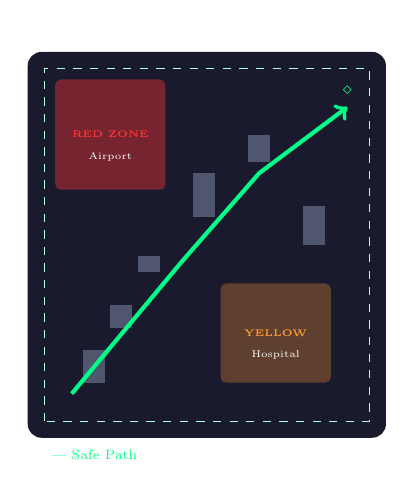
\begin{tikzpicture}[scale=0.7, transform shape]
    % City representation
    \fill[cardbg, rounded corners=5pt] (0,0) rectangle (6.5,7);
    \draw[neongreen!30, dashed] (0.3,0.3) rectangle (6.2,6.7);
    
    % Red zone
    \fill[dangerred, opacity=0.4, rounded corners=2pt] (0.5,4.5) rectangle (2.5,6.5);
    \node[font=\tiny, text=dangerred] at (1.5,5.5) {\textbf{RED ZONE}};
    \node[font=\tiny, text=white] at (1.5,5.1) {Airport};
    
    % Yellow zone
    \fill[warnorange, opacity=0.3, rounded corners=2pt] (3.5,1.0) rectangle (5.5,2.8);
    \node[font=\tiny, text=warnorange] at (4.5,1.9) {\textbf{YELLOW}};
    \node[font=\tiny, text=white] at (4.5,1.5) {Hospital};
    
    % Buildings
    \foreach \x/\y/\h in {1/1/0.6, 1.5/2/0.4, 3/4/0.8, 4/5/0.5, 5/3.5/0.7, 2/3/0.3} {
        \fill[softgray, opacity=0.5] (\x,\y) rectangle ++(0.4,\h);
    }
    
    % Drone path
    \draw[neongreen, line width=1.5pt, ->] (0.8,0.8) -- (2.8,3.2) -- (4.2,4.8) -- (5.8,6.0);
    
    % Drone icon
    \node[font=\small] at (5.8,6.3) {\textcolor{neongreen}{$\diamond$}};
    
    % Legend
    \node[font=\scriptsize, text=neongreen, anchor=west] at (0.3,-0.3) {--- Safe Path};
    \node[font=\scriptsize, text=white] at (3.25,7.2) {\textbf{Jaipur Airspace (20$\times$20 km)}};
\end{tikzpicture}
\end{column}
\end{columns}
\end{frame}

% ═══════════════════════════════════════
% SLIDE 4: OBJECTIVES
% ═══════════════════════════════════════
\begin{frame}{Project Objectives}
\begin{center}
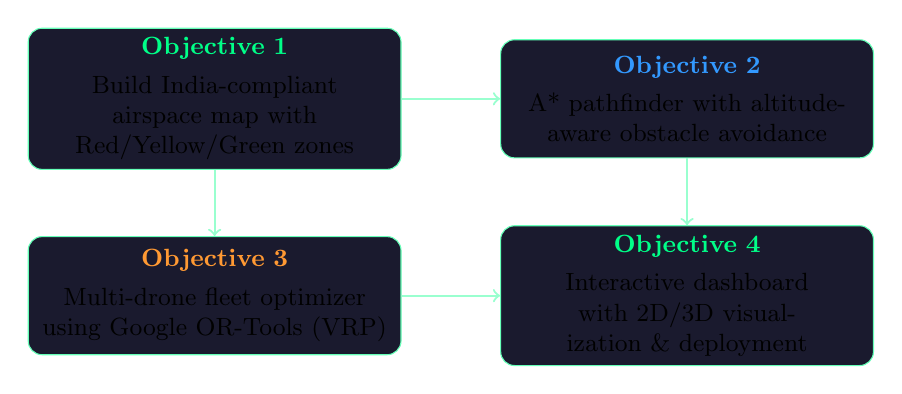
\begin{tikzpicture}[
    obj/.style={rectangle, draw=neongreen!60, fill=cardbg, text width=4.5cm, text centered, rounded corners=5pt, minimum height=1.5cm, font=\small},
]
    \node[obj] (o1) at (0,3) {\textcolor{neongreen}{\textbf{Objective 1}}\\[0.1cm] Build India-compliant airspace map with Red/Yellow/Green zones};
    \node[obj] (o2) at (6,3) {\textcolor{accentblue}{\textbf{Objective 2}}\\[0.1cm] A* pathfinder with altitude-aware obstacle avoidance};
    \node[obj] (o3) at (0,0.5) {\textcolor{warnorange}{\textbf{Objective 3}}\\[0.1cm] Multi-drone fleet optimizer using Google OR-Tools (VRP)};
    \node[obj] (o4) at (6,0.5) {\textcolor{neongreen}{\textbf{Objective 4}}\\[0.1cm] Interactive dashboard with 2D/3D visualization \& deployment};
    
    \draw[neongreen!40, ->, thick] (o1) -- (o2);
    \draw[neongreen!40, ->, thick] (o2) -- (o4);
    \draw[neongreen!40, ->, thick] (o1) -- (o3);
    \draw[neongreen!40, ->, thick] (o3) -- (o4);
\end{tikzpicture}
\end{center}
\end{frame}

% ═══════════════════════════════════════
% SLIDE 5: LITERATURE REVIEW
% ═══════════════════════════════════════
\begin{frame}{Literature Review}
\small
\begin{tabular}{@{}p{2.5cm}p{3.5cm}p{3.0cm}p{3.5cm}@{}}
\toprule
\textcolor{neongreen}{\textbf{Approach}} & \textcolor{neongreen}{\textbf{Strengths}} & \textcolor{dangerred}{\textbf{Weaknesses}} & \textcolor{accentblue}{\textbf{Refs}} \\
\midrule
\textbf{Potential Fields} & Simple, real-time & Local minima & Khatib, 1986 \\[0.2cm]
\textbf{A* Search} & Optimal, complete, fast & Grid-dependent & Hart et al., 1968 \\[0.2cm]
\textbf{RRT*} & High-dim, any space & Non-deterministic & Karaman, 2011 \\[0.2cm]
\textbf{Jump Point} & Faster than A* & Uniform grids only & Harabor, 2011 \\[0.2cm]
\textbf{VRP Solvers} & Fleet optimization & NP-hard scaling & Dantzig, 1959 \\
\bottomrule
\end{tabular}

\vspace{0.4cm}
\begin{alertblock}{Research Gap}
No existing work combines \textbf{India-specific regulatory zones} (Red/Yellow) + \textbf{altitude-aware building avoidance} + \textbf{multi-drone fleet optimization} in a single deployable system.
\end{alertblock}
\end{frame}

% ═══════════════════════════════════════
% SLIDE 6: SYSTEM ARCHITECTURE
% ═══════════════════════════════════════
\begin{frame}{System Architecture -- 8-Stage Pipeline}
\begin{center}
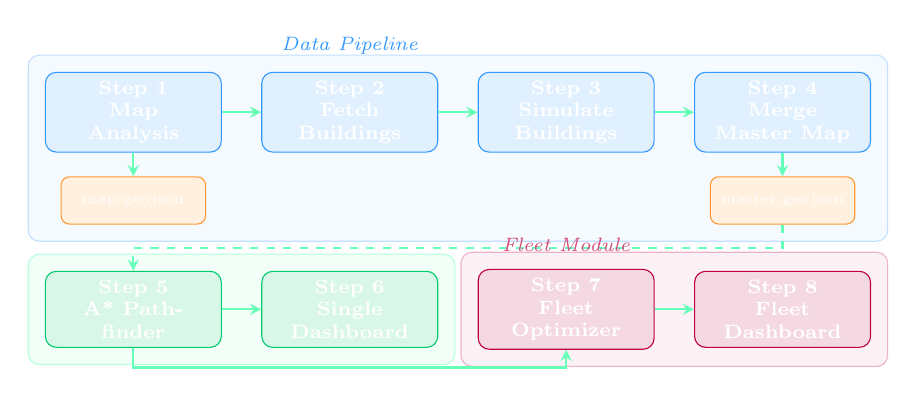
\begin{tikzpicture}[
    node distance=0.6cm and 0.5cm,
    block/.style={rectangle, draw=#1, fill=#1!15, text width=2.0cm, text centered, rounded corners=4pt, minimum height=0.9cm, font=\scriptsize\bfseries, text=white},
    data/.style={rectangle, draw=warnorange, fill=warnorange!15, text width=1.6cm, text centered, rounded corners=3pt, minimum height=0.6cm, font=\tiny, text=white},
    arr/.style={->, >=stealth, thick, draw=neongreen!60},
]
% Row 1
\node[block=accentblue] (s1) {Step 1\\Map\\Analysis};
\node[block=accentblue, right=of s1] (s2) {Step 2\\Fetch\\Buildings};
\node[block=accentblue, right=of s2] (s3) {Step 3\\Simulate\\Buildings};
\node[block=accentblue, right=of s3] (s4) {Step 4\\Merge\\Master Map};

% Data
\node[data, below=0.3cm of s1] (d1) {map.geojson};
\node[data, below=0.3cm of s4] (d4) {master.geojson};

% Row 2
\node[block=neongreen!80!black, below=1.5cm of s1] (s5) {Step 5\\A* Path-\\finder};
\node[block=neongreen!80!black, right=of s5] (s6) {Step 6\\Single\\Dashboard};
\node[block=purple, right=of s6] (s7) {Step 7\\Fleet\\Optimizer};
\node[block=purple, right=of s7] (s8) {Step 8\\Fleet\\Dashboard};

% Arrows
\draw[arr] (s1) -- (s2);
\draw[arr] (s2) -- (s3);
\draw[arr] (s3) -- (s4);
\draw[arr] (s1) -- (d1);
\draw[arr] (s4) -- (d4);
\draw[arr, dashed] (d4.south) -- ++(0,-0.3) -| (s5.north);
\draw[arr] (s5) -- (s6);
\draw[arr] (s5.south) -- ++(0,-0.25) -| (s7.south);
\draw[arr] (s7) -- (s8);

% Labels
\node[above=0.1cm of s2, font=\scriptsize\itshape, text=accentblue] {Data Pipeline};
\node[above=0.1cm of s7, font=\scriptsize\itshape, text=purple!70] {Fleet Module};

% Grouping
\scoped[on background layer] {
    \node[draw=accentblue!30, fill=accentblue!5, rounded corners, inner sep=6pt, fit=(s1)(s4)(d1)(d4)] {};
    \node[draw=neongreen!30, fill=neongreen!5, rounded corners, inner sep=6pt, fit=(s5)(s6)] {};
    \node[draw=purple!30, fill=purple!5, rounded corners, inner sep=6pt, fit=(s7)(s8)] {};
}
\end{tikzpicture}
\end{center}

\vspace{0.2cm}
\begin{columns}[T]
\begin{column}{0.3\textwidth}
\begin{exampleblock}{\footnotesize Data Layer}
\footnotesize GeoJSON zones + OSMnx buildings + Gaussian simulation
\end{exampleblock}
\end{column}
\begin{column}{0.3\textwidth}
\begin{exampleblock}{\footnotesize Engine Layer}
\footnotesize A* pathfinding with octile heuristic + string-pulling
\end{exampleblock}
\end{column}
\begin{column}{0.3\textwidth}
\begin{exampleblock}{\footnotesize Fleet Layer}
\footnotesize OR-Tools VRP with capacity + battery constraints
\end{exampleblock}
\end{column}
\end{columns}
\end{frame}

% ═══════════════════════════════════════
% SLIDE 7: TECHNOLOGY STACK
% ═══════════════════════════════════════
\begin{frame}{Technology Stack}
\begin{columns}[T]
\begin{column}{0.48\textwidth}
\begin{block}{Core Technologies}
\small
\begin{tabular}{@{}ll@{}}
\textcolor{neongreen}{$\blacksquare$} Language & Python 3.13 \\
\textcolor{neongreen}{$\blacksquare$} GIS & GeoPandas, Shapely \\
\textcolor{neongreen}{$\blacksquare$} Buildings & OSMnx \\
\textcolor{neongreen}{$\blacksquare$} Pathfinding & Custom A* \\
\textcolor{neongreen}{$\blacksquare$} Fleet & Google OR-Tools \\
\textcolor{neongreen}{$\blacksquare$} Math & NumPy, SciPy \\
\end{tabular}
\end{block}
\vspace{0.2cm}
\begin{block}{Frontend \& Deploy}
\small
\begin{tabular}{@{}ll@{}}
\textcolor{accentblue}{$\blacksquare$} Dashboard & Streamlit 1.45 \\
\textcolor{accentblue}{$\blacksquare$} 2D Maps & Folium 0.15 \\
\textcolor{accentblue}{$\blacksquare$} 3D Maps & PyDeck 0.8 \\
\textcolor{accentblue}{$\blacksquare$} Hosting & HuggingFace \\
\end{tabular}
\end{block}
\end{column}
\begin{column}{0.48\textwidth}
\begin{center}
\begin{tikzpicture}[scale=0.8, transform shape]
    % Stack visualization
    \foreach \i/\name/\col in {0/Hugging Face Spaces/accentblue, 1/Streamlit Dashboard/neongreen!80!black, 2/Folium + PyDeck (Viz)/accentblue, 3/OR-Tools (Fleet)/purple!80, 4/A* Pathfinder/neongreen!80!black, 5/GeoPandas + OSMnx/warnorange, 6/Python 3.13/softgray} {
        \fill[\col!30, rounded corners=3pt] (0,\i*0.8) rectangle (5.5, \i*0.8+0.65);
        \draw[\col, rounded corners=3pt] (0,\i*0.8) rectangle (5.5, \i*0.8+0.65);
        \node[font=\scriptsize\bfseries, text=white] at (2.75, \i*0.8+0.325) {\name};
    }
    \node[font=\tiny\itshape, text=softgray] at (2.75, -0.3) {Technology Stack (Bottom to Top)};
\end{tikzpicture}
\end{center}
\end{column}
\end{columns}
\end{frame}

% ═══════════════════════════════════════
% SLIDE 8: STEP 1-2 MAP & BUILDINGS
% ═══════════════════════════════════════
\begin{frame}{Step 1--2: Map Analysis \& Building Fetch}
\begin{columns}[T]
\begin{column}{0.50\textwidth}
\textcolor{neongreen}{\textbf{Step 1: Airspace Classification}}\\[0.2cm]
\small
Custom GeoJSON map encoding Jaipur airspace:
\begin{itemize}
    \item[\textcolor{dangerred}{$\blacksquare$}] \textbf{12 Red Zones} -- No-fly (airports, military)\\Height: 500m $\rightarrow$ guaranteed A* avoidance
    \item[\textcolor{warnorange}{$\blacksquare$}] \textbf{20 Yellow Zones} -- Conditional (hospitals, schools)\\Require operator permission
    \item[\textcolor{neongreen}{$\blacksquare$}] \textbf{Boundary} -- 20$\times$20 km operational area
\end{itemize}

\vspace{0.3cm}
\textcolor{accentblue}{\textbf{Step 2: OSMnx Building Fetch}}\\[0.2cm]
\small
\begin{itemize}
    \item Query OpenStreetMap for Jaipur buildings
    \item Extract footprint polygons + metadata
    \item Assign realistic heights where missing
\end{itemize}
\end{column}
\begin{column}{0.45\textwidth}
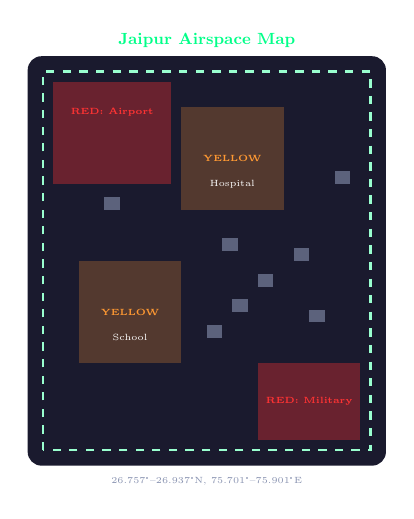
\begin{tikzpicture}[scale=0.65, transform shape]
    % Map container
    \fill[cardbg, rounded corners=5pt] (0,0) rectangle (7,8);
    \draw[neongreen!40, dashed, thick] (0.3,0.3) rectangle (6.7,7.7);
    
    % Red zones
    \fill[dangerred, opacity=0.35] (0.5,5.5) rectangle (2.8,7.5);
    \node[font=\tiny\bfseries, text=dangerred] at (1.65,6.9) {RED: Airport};
    
    \fill[dangerred, opacity=0.35] (4.5,0.5) rectangle (6.5,2.0);
    \node[font=\tiny\bfseries, text=dangerred] at (5.5,1.25) {RED: Military};
    
    % Yellow zones
    \fill[warnorange, opacity=0.25] (3.0,5.0) rectangle (5.0,7.0);
    \node[font=\tiny\bfseries, text=warnorange] at (4.0,6.0) {YELLOW};
    \node[font=\tiny, text=white] at (4.0,5.5) {Hospital};
    
    \fill[warnorange, opacity=0.25] (1.0,2.0) rectangle (3.0,4.0);
    \node[font=\tiny\bfseries, text=warnorange] at (2.0,3.0) {YELLOW};
    \node[font=\tiny, text=white] at (2.0,2.5) {School};
    
    % Buildings
    \foreach \x/\y in {3.5/2.5, 4.0/3.0, 4.5/3.5, 3.8/4.2, 5.2/4.0, 5.5/2.8, 1.5/5.0, 6.0/5.5} {
        \fill[softgray, opacity=0.6] (\x,\y) rectangle ++(0.3,0.25);
    }
    
    % Title
    \node[font=\small\bfseries, text=neongreen] at (3.5,8.3) {Jaipur Airspace Map};
    \node[font=\tiny, text=softgray] at (3.5, -0.3) {26.757°--26.937°N, 75.701°--75.901°E};
\end{tikzpicture}
\end{column}
\end{columns}
\end{frame}

% ═══════════════════════════════════════
% SLIDE 9: STEP 3-4 BUILDING SIMULATION
% ═══════════════════════════════════════
\begin{frame}{Step 3--4: Building Simulation \& Master Map}
\begin{columns}[T]
\begin{column}{0.50\textwidth}
\textcolor{neongreen}{\textbf{Step 3: Gaussian Building Generation}}\\[0.2cm]
\small
\begin{itemize}
    \item \textbf{1,079 buildings} procedurally generated
    \item Gaussian cluster density model:
\end{itemize}
$$P(x,y) = \sum_{k=1}^{K} \frac{w_k}{2\pi\sigma^2} e^{-\frac{(x-\mu_k)^2 + (y-\mu_k)^2}{2\sigma^2}}$$
\begin{itemize}
    \item Heights: $\mathcal{N}(45, 10)$ truncated to $[30, 60]$\,m
    \item Min gap: 18\,m between buildings
    \item 8 cluster centers across Jaipur
\end{itemize}

\vspace{0.3cm}
\textcolor{accentblue}{\textbf{Step 4: Master Map Merge}}\\[0.2cm]
\small
\begin{itemize}
    \item Merge zones + buildings $\rightarrow$ \texttt{master\_map.geojson}
    \item Each feature has \texttt{height} attribute
    \item Red zones: 500m, Yellow: 400m
\end{itemize}
\end{column}
\begin{column}{0.45\textwidth}
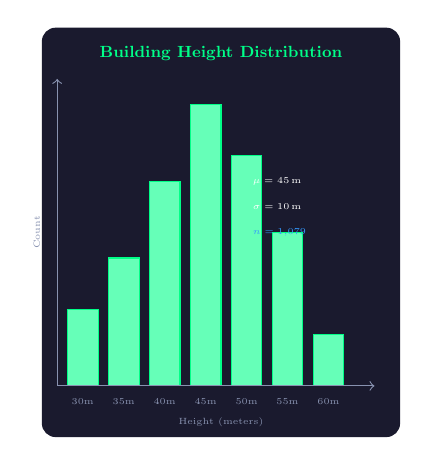
\begin{tikzpicture}[scale=0.65, transform shape]
    % Building height distribution
    \fill[cardbg, rounded corners=5pt] (0,0) rectangle (7,8);
    \node[font=\small\bfseries, text=neongreen] at (3.5,7.5) {Building Height Distribution};
    
    % Histogram bars
    \foreach \x/\h/\lab in {0.5/1.5/30, 1.3/2.5/35, 2.1/4.0/40, 2.9/5.5/45, 3.7/4.5/50, 4.5/3.0/55, 5.3/1.0/60} {
        \fill[neongreen!60] (\x,1.0) rectangle ++(0.6,\h);
        \draw[neongreen] (\x,1.0) rectangle ++(0.6,\h);
        \node[font=\tiny, text=softgray, rotate=0] at (\x+0.3,0.7) {\lab m};
    }
    
    % Axis
    \draw[softgray, ->] (0.3,1.0) -- (6.5,1.0);
    \draw[softgray, ->] (0.3,1.0) -- (0.3,7.0);
    \node[font=\tiny, text=softgray] at (3.5,0.3) {Height (meters)};
    \node[font=\tiny, text=softgray, rotate=90] at (-0.1,4.0) {Count};
    
    % Stats
    \node[font=\tiny, text=white, anchor=west] at (4.0,5.0) {$\mu = 45$\,m};
    \node[font=\tiny, text=white, anchor=west] at (4.0,4.5) {$\sigma = 10$\,m};
    \node[font=\tiny, text=accentblue, anchor=west] at (4.0,4.0) {$n = 1{,}079$};
\end{tikzpicture}
\end{column}
\end{columns}
\end{frame}

% ═══════════════════════════════════════
% SLIDE 10: STEP 5 A* PATHFINDING
% ═══════════════════════════════════════
\begin{frame}{Step 5: A* Pathfinding Engine}
\begin{columns}[T]
\begin{column}{0.50\textwidth}
\textcolor{neongreen}{\textbf{Grid Discretization}}
\small
\begin{itemize}
    \item 401 $\times$ 400 grid = \textbf{160,400 cells}
    \item Resolution: $\sim$50m per cell
    \item 8-directional movement
\end{itemize}

\vspace{0.2cm}
\textcolor{accentblue}{\textbf{A* Formula}}
$$f(n) = g(n) + h(n)$$

\textbf{Octile Heuristic} (admissible + consistent):
$$h(n) = D_{\max} + (\sqrt{2}-1) \cdot D_{\min}$$

\vspace{0.2cm}
\textcolor{warnorange}{\textbf{Cell Blocking Rule}}
\small
{\footnotesize
$$\text{blocked}(c) = \begin{cases} \text{T}, & c \in \text{RedZone} \cup \text{YellowZone}^{\neg p} \\ \text{T}, & h(c) \geq h_{\text{drone}} - m_s \\ \text{F}, & \text{otherwise}\end{cases}$$
}
\end{column}
\begin{column}{0.45\textwidth}
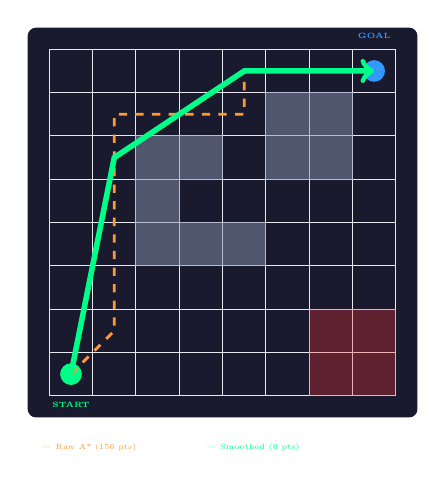
\begin{tikzpicture}[scale=0.55, transform shape]
    % Grid
    \fill[cardbg, rounded corners=3pt] (-0.5,-0.5) rectangle (8.5,8.5);
    
    % Grid lines
    \foreach \i in {0,...,8} {
        \draw[softgray!20] (\i,0) -- (\i,8);
        \draw[softgray!20] (0,\i) -- (8,\i);
    }
    
    % Obstacles (buildings)
    \foreach \x/\y in {2/3, 2/4, 2/5, 3/5, 3/3, 4/3, 5/5, 5/6, 6/5, 6/6} {
        \fill[softgray, opacity=0.5] (\x,\y) rectangle ++(1,1);
        \draw[softgray!60] (\x,\y) rectangle ++(1,1);
    }
    
    % Red zone
    \fill[dangerred, opacity=0.3] (6,0) rectangle (8,2);
    
    % Start
    \fill[neongreen] (0.5,0.5) circle (0.25);
    \node[font=\tiny\bfseries, text=neongreen] at (0.5,-0.2) {START};
    
    % End
    \fill[accentblue] (7.5,7.5) circle (0.25);
    \node[font=\tiny\bfseries, text=accentblue] at (7.5,8.3) {GOAL};
    
    % Path (raw A*)
    \draw[warnorange, line width=1pt, dashed] (0.5,0.5) -- (1.5,1.5) -- (1.5,2.5) -- (1.5,3.5) -- (1.5,4.5) -- (1.5,5.5) -- (1.5,6.5) -- (2.5,6.5) -- (3.5,6.5) -- (4.5,6.5) -- (4.5,7.5) -- (5.5,7.5) -- (6.5,7.5) -- (7.5,7.5);
    
    % Smoothed path
    \draw[neongreen, line width=2pt, ->] (0.5,0.5) -- (1.5,5.5) -- (4.5,7.5) -- (7.5,7.5);
    
    % Legend
    \node[font=\tiny, text=warnorange, anchor=west] at (-0.3,-1.2) {--- Raw A* (156 pts)};
    \node[font=\tiny, text=neongreen, anchor=west] at (3.5,-1.2) {--- Smoothed (6 pts)};
\end{tikzpicture}
\end{column}
\end{columns}
\end{frame}

% ═══════════════════════════════════════
% SLIDE 11: STRING PULLING
% ═══════════════════════════════════════
\begin{frame}{A* Path Smoothing: String-Pulling Algorithm}
\begin{columns}[T]
\begin{column}{0.55\textwidth}
\textcolor{neongreen}{\textbf{Problem:}} Raw A* produces jagged, grid-aligned paths (150+ waypoints)\\[0.3cm]

\textcolor{accentblue}{\textbf{Solution:}} String-pulling with ray-marching\\[0.2cm]
\small
\begin{enumerate}
    \item Start from first waypoint
    \item Try straight line to \textbf{farthest} subsequent waypoint
    \item If line is \textbf{obstacle-free} $\rightarrow$ skip intermediates
    \item Advance to farthest visible point, repeat
\end{enumerate}

\vspace{0.3cm}
\begin{exampleblock}{Result}
\footnotesize
\textbf{96\% waypoint reduction} on average\\
156 waypoints $\rightarrow$ 6 smooth flight vectors
\end{exampleblock}
\end{column}
\begin{column}{0.43\textwidth}
\small
\begin{tabular}{@{}lccc@{}}
\toprule
\textcolor{neongreen}{\textbf{Mission}} & \textbf{Raw} & \textbf{Smooth} & \textbf{Cut} \\
\midrule
M1 (N$\to$S) & 156 & 6 & 96\% \\
M2 (E$\to$W) & 98 & 5 & 95\% \\
M3 (Cross) & 243 & 8 & 97\% \\
M4 (Dense) & 72 & 4 & 94\% \\
\bottomrule
\end{tabular}
\vspace{0.3cm}

\textcolor{warnorange}{\textbf{Why it matters:}}
\begin{itemize}\footnotesize
    \item Fewer waypoints = smoother flight
    \item Less onboard memory needed
    \item Direct flight vectors for autopilot
\end{itemize}
\end{column}
\end{columns}
\end{frame}

% ═══════════════════════════════════════
% SLIDE 12: ALTITUDE AWARENESS
% ═══════════════════════════════════════
\begin{frame}{Altitude-Aware Obstacle Avoidance}
\begin{columns}[T]
\begin{column}{0.50\textwidth}
\textcolor{neongreen}{\textbf{Key Insight:}} Not all buildings are obstacles!\\[0.3cm]
\small
A drone at 60m altitude with 10m safety margin:\\
$\rightarrow$ \textbf{Threshold = 50m}\\
$\rightarrow$ Buildings $<$ 50m are \textbf{ignored}\\
$\rightarrow$ Buildings $\geq$ 50m are \textbf{avoided}

\vspace{0.4cm}
\begin{tabular}{@{}cccc@{}}
\toprule
\textcolor{neongreen}{\textbf{Alt}} & \textcolor{accentblue}{\textbf{Safety}} & \textcolor{warnorange}{\textbf{Thresh}} & \textbf{Blocked} \\
\midrule
40\,m & 10\,m & 30\,m & 1,079 \\
\rowcolor{neongreen!10}
60\,m & 10\,m & 50\,m & 412 \\
80\,m & 10\,m & 70\,m & 0 \\
60\,m & 0\,m & 60\,m & 89 \\
\bottomrule
\end{tabular}
\end{column}
\begin{column}{0.45\textwidth}
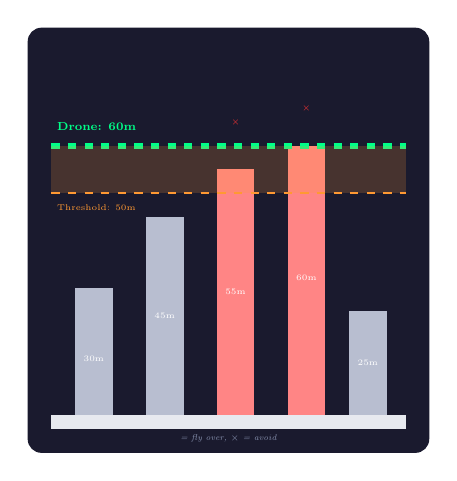
\begin{tikzpicture}[scale=0.6, transform shape]
    \fill[cardbg, rounded corners=5pt] (-0.5,-0.5) rectangle (8,8.5);
    
    % Ground
    \fill[softgray!20] (0,0) rectangle (7.5,0.3);
    
    % Buildings with heights
    \fill[softgray!60] (0.5,0.3) rectangle (1.3,3.0);
    \node[font=\tiny, text=white] at (0.9,1.5) {30m};
    
    \fill[softgray!60] (2.0,0.3) rectangle (2.8,4.5);
    \node[font=\tiny, text=white] at (2.4,2.4) {45m};
    
    \fill[dangerred!60] (3.5,0.3) rectangle (4.3,5.5);
    \node[font=\tiny, text=white] at (3.9,2.9) {55m};
    
    \fill[dangerred!60] (5.0,0.3) rectangle (5.8,6.0);
    \node[font=\tiny, text=white] at (5.4,3.2) {60m};
    
    \fill[softgray!60] (6.3,0.3) rectangle (7.1,2.5);
    \node[font=\tiny, text=white] at (6.7,1.4) {25m};
    
    % Drone altitude line
    \draw[neongreen, line width=2pt, dashed] (0,6.0) -- (7.5,6.0);
    \node[font=\scriptsize\bfseries, text=neongreen, anchor=west] at (0,6.4) {Drone: 60m};
    
    % Safety margin
    \fill[warnorange, opacity=0.2] (0,5.0) rectangle (7.5,6.0);
    \draw[warnorange, dashed] (0,5.0) -- (7.5,5.0);
    \node[font=\tiny, text=warnorange, anchor=west] at (0,4.7) {Threshold: 50m};
    
    % Labels
    \node[font=\tiny, text=neongreen] at (0.9,3.5) {\checkmark};
    \node[font=\tiny, text=neongreen] at (2.4,5.0) {\checkmark};
    \node[font=\tiny, text=dangerred] at (3.9,6.5) {$\times$};
    \node[font=\tiny, text=dangerred] at (5.4,6.8) {$\times$};
    \node[font=\tiny, text=neongreen] at (6.7,3.0) {\checkmark};
    
    \node[font=\tiny\itshape, text=softgray] at (3.75,-0.2) {\checkmark = fly over, $\times$ = avoid};
\end{tikzpicture}
\end{column}
\end{columns}
\end{frame}

% ═══════════════════════════════════════
% SLIDE 13: CONFIGURABLE PARAMETERS
% ═══════════════════════════════════════
\begin{frame}{Operator-Configurable Parameters}
\begin{columns}[T]
\begin{column}{0.55\textwidth}
\small
All parameters are \textbf{live-adjustable} via dashboard sidebar:

\vspace{0.3cm}
\begin{tabular}{@{}p{2.2cm}p{1.5cm}p{1.0cm}p{2.0cm}@{}}
\toprule
\textcolor{neongreen}{\textbf{Param}} & \textbf{Range} & \textbf{Default} & \textbf{Effect} \\
\midrule
Altitude & 20--120m & 60m & Cruise height \\
Speed & 10--100 & 50 km/h & Time est. \\
Vert.\ Margin & 0--30m & 10m & Above-bldg \\
Bldg.\ Buffer & 0--20m & 3m & Lateral gap \\
Capacity & 0.5--20kg & 2.5kg & Payload \\
Battery & Fixed & 3 km/\% & Discharge \\
\bottomrule
\end{tabular}

\vspace{0.3cm}
\textcolor{accentblue}{\textbf{Building Buffer:}} Expands footprints horizontally before grid marking $\rightarrow$ ensures lateral safety clearance.

\vspace{0.2cm}
\textcolor{warnorange}{\textbf{Battery Model:}} 3\,km per 1\% $\rightarrow$ 300\,km max range at full charge.
\end{column}
\begin{column}{0.42\textwidth}
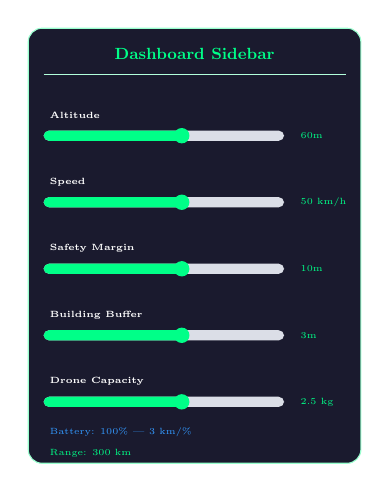
\begin{tikzpicture}[scale=0.65, transform shape]
    % Sidebar mockup
    \fill[cardbg, rounded corners=5pt] (0,0) rectangle (6.5,8.5);
    \draw[neongreen!40, rounded corners=5pt] (0,0) rectangle (6.5,8.5);
    
    \node[font=\small\bfseries, text=neongreen] at (3.25,8.0) {Dashboard Sidebar};
    \draw[neongreen!30] (0.3,7.6) -- (6.2,7.6);
    
    % Sliders
    \foreach \i/\name/\val in {0/Altitude/60m, 1/Speed/50 km\slash h, 2/Safety Margin/10m, 3/Building Buffer/3m, 4/Drone Capacity/2.5 kg} {
        \pgfmathsetmacro\ypos{6.8 - \i*1.3}
        \node[font=\tiny\bfseries, text=white, anchor=west] at (0.3,\ypos) {\name};
        \fill[softgray!30, rounded corners=2pt] (0.3,\ypos-0.5) rectangle (5.0,\ypos-0.3);
        \fill[neongreen, rounded corners=2pt] (0.3,\ypos-0.5) rectangle (3.0,\ypos-0.3);
        \fill[neongreen] (3.0,\ypos-0.4) circle (0.15);
        \node[font=\tiny, text=neongreen, anchor=west] at (5.2,\ypos-0.4) {\val};
    }
    
    % Battery info
    \node[font=\tiny, text=accentblue, anchor=west] at (0.3,0.6) {Battery: 100\% | 3 km/\%};
    \node[font=\tiny, text=neongreen, anchor=west] at (0.3,0.2) {Range: 300 km};
\end{tikzpicture}
\end{column}
\end{columns}
\end{frame}

% ═══════════════════════════════════════
% SLIDE 14: STEP 6 DASHBOARD
% ═══════════════════════════════════════
\begin{frame}{Step 6: Single Drone Dashboard}
\begin{columns}[T]
\begin{column}{0.50\textwidth}
\textcolor{neongreen}{\textbf{Features:}}
\begin{itemize}\small
    \item[\textcolor{neongreen}{$\bullet$}] \textbf{Point \& Click} -- set pickup/drop on map
    \item[\textcolor{neongreen}{$\bullet$}] \textbf{Manual Entry} -- lat/lon input
    \item[\textcolor{neongreen}{$\bullet$}] \textbf{Yellow Zone Selector} -- permit/deny per zone
    \item[\textcolor{neongreen}{$\bullet$}] \textbf{2D Map} -- Folium with zones + buildings + path
    \item[\textcolor{neongreen}{$\bullet$}] \textbf{3D Map} -- PyDeck with extruded buildings
    \item[\textcolor{neongreen}{$\bullet$}] \textbf{Metrics} -- distance, time, battery, compliance
\end{itemize}

\vspace{0.3cm}
\begin{exampleblock}{Sample Results}
\footnotesize
\begin{tabular}{@{}lccc@{}}
\toprule
\textbf{Mission} & \textbf{Dist} & \textbf{Time} & \textbf{Compute} \\
\midrule
N$\to$S & 9.47 km & 11.4 min & 47 ms \\
Cross-city & 15.83 km & 19.0 min & 89 ms \\
\bottomrule
\end{tabular}
\end{exampleblock}
\end{column}
\begin{column}{0.45\textwidth}
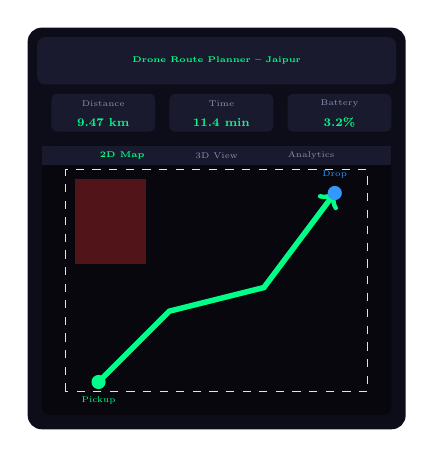
\begin{tikzpicture}[scale=0.6, transform shape]
    % Dashboard mockup
    \fill[darkbg, rounded corners=5pt] (0,0) rectangle (8,8.5);
    
    % Header
    \fill[cardbg, rounded corners=3pt] (0.2,7.3) rectangle (7.8,8.3);
    \node[font=\tiny\bfseries, text=neongreen] at (4,7.8) {Drone Route Planner -- Jaipur};
    
    % Metrics row
    \foreach \i/\val/\lab in {0/9.47 km/Distance, 1/11.4 min/Time, 2/3.2\%/Battery} {
        \pgfmathsetmacro\xpos{0.5 + \i*2.5}
        \fill[cardbg, rounded corners=2pt] (\xpos,6.3) rectangle ++(2.2,0.8);
        \node[font=\tiny, text=softgray] at (\xpos+1.1,6.9) {\lab};
        \node[font=\scriptsize\bfseries, text=neongreen] at (\xpos+1.1,6.5) {\val};
    }
    
    % Map area
    \fill[darkbg!50!black, rounded corners=3pt] (0.3,0.3) rectangle (7.7,6.0);
    \draw[neongreen!30, dashed] (0.8,0.8) rectangle (7.2,5.5);
    
    % Red zone
    \fill[dangerred, opacity=0.3] (1.0,3.5) rectangle (2.5,5.3);
    
    % Path
    \draw[neongreen, line width=2pt, ->] (1.5,1.0) -- (3.0,2.5) -- (5.0,3.0) -- (6.5,5.0);
    
    % Points
    \fill[neongreen] (1.5,1.0) circle (0.15);
    \fill[accentblue] (6.5,5.0) circle (0.15);
    \node[font=\tiny, text=neongreen] at (1.5,0.6) {Pickup};
    \node[font=\tiny, text=accentblue] at (6.5,5.4) {Drop};
    
    % Tab bar
    \fill[cardbg] (0.3,5.6) rectangle (7.7,6.0);
    \node[font=\tiny\bfseries, text=neongreen] at (2.0,5.8) {2D Map};
    \node[font=\tiny, text=softgray] at (4.0,5.8) {3D View};
    \node[font=\tiny, text=softgray] at (6.0,5.8) {Analytics};
\end{tikzpicture}
\end{column}
\end{columns}
\end{frame}

% ═══════════════════════════════════════
% SLIDE 15: STEP 7 FLEET OPTIMIZATION
% ═══════════════════════════════════════
\begin{frame}{Step 7: Fleet Optimization with Google OR-Tools}
\begin{columns}[T]
\begin{column}{0.50\textwidth}
\textcolor{neongreen}{\textbf{Vehicle Routing Problem (VRP)}}\\[0.2cm]
\small
Minimize total fleet distance:
$$\min \sum_{k=1}^{M} \sum_{(i,j) \in \mathcal{R}_k} C_{ij}$$

\textbf{Subject to:}
\begin{itemize}\footnotesize
    \item[\textcolor{neongreen}{1.}] Weight per drone $\leq$ capacity
    \item[\textcolor{neongreen}{2.}] Distance per drone $\leq$ battery range
    \item[\textcolor{neongreen}{3.}] Each drop visited \textbf{exactly once}
    \item[\textcolor{neongreen}{4.}] All routes start/end at warehouse
\end{itemize}

\vspace{0.2cm}
\textcolor{accentblue}{\textbf{Cost Matrix:}}\\
\footnotesize
$C_{ij}$ = A*-safe distance between locations $i,j$\\
Requires $\binom{N}{2}$ A* computations\\[0.2cm]
\textcolor{warnorange}{\textbf{Solver:}} PATH\_CHEAPEST\_ARC + GUIDED\_LOCAL\_SEARCH
\end{column}
\begin{column}{0.45\textwidth}
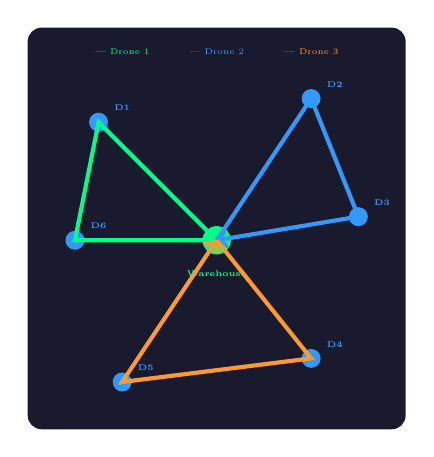
\begin{tikzpicture}[scale=0.6, transform shape]
    \fill[cardbg, rounded corners=5pt] (0,0) rectangle (8,8.5);
    
    % Warehouse
    \fill[neongreen] (4,4) circle (0.3);
    \node[font=\tiny\bfseries, text=neongreen] at (4,3.3) {Warehouse};
    
    % Drop points
    \foreach \x/\y/\n in {1.5/6.5/D1, 6/7/D2, 7/4.5/D3, 6/1.5/D4, 2/1/D5, 1/4/D6} {
        \fill[accentblue] (\x,\y) circle (0.2);
        \node[font=\tiny\bfseries, text=accentblue] at (\x+0.5,\y+0.3) {\n};
    }
    
    % Drone 1 route (green)
    \draw[neongreen, line width=1.5pt, ->] (4,4) -- (1.5,6.5) -- (1,4) -- (4,4);
    
    % Drone 2 route (blue)  
    \draw[accentblue, line width=1.5pt, ->] (4,4) -- (6,7) -- (7,4.5) -- (4,4);
    
    % Drone 3 route (orange)
    \draw[warnorange, line width=1.5pt, ->] (4,4) -- (6,1.5) -- (2,1) -- (4,4);
    
    % Legend
    \node[font=\tiny, text=neongreen] at (2,8.0) {--- Drone 1};
    \node[font=\tiny, text=accentblue] at (4,8.0) {--- Drone 2};
    \node[font=\tiny, text=warnorange] at (6,8.0) {--- Drone 3};
\end{tikzpicture}
\end{column}
\end{columns}
\end{frame}

% ═══════════════════════════════════════
% SLIDE 16: COST MATRIX
% ═══════════════════════════════════════
\begin{frame}{Cost Matrix Construction}
\begin{columns}[T]
\begin{column}{0.50\textwidth}
\textcolor{neongreen}{\textbf{How Cost Matrix is Built:}}\\[0.2cm]
\small
\begin{enumerate}
    \item Build obstacle grid from master map
    \item For every pair of locations $(i, j)$:
        \begin{itemize}\footnotesize
            \item Run A* pathfinder
            \item Store safe-path distance in $C_{ij}$
        \end{itemize}
    \item Pass matrix $\mathbf{C}$ to OR-Tools
\end{enumerate}

\vspace{0.3cm}
\textcolor{accentblue}{\textbf{Key Properties:}}
\begin{itemize}\small
    \item Symmetric: $C_{ij} = C_{ji}$
    \item All paths avoid obstacles
    \item $C_{ij} \geq$ Haversine distance (always)
    \item For $N=7$: $\binom{7}{2} = 21$ A* runs
\end{itemize}

\vspace{0.2cm}
\textcolor{warnorange}{\textbf{Not}} Euclidean distance -- \textbf{safe-path distance!}
\end{column}
\begin{column}{0.45\textwidth}
\small
\textcolor{neongreen}{\textbf{Example Cost Matrix (km):}}\\[0.2cm]
\footnotesize
\begin{tabular}{@{}lcccc@{}}
\toprule
& \textbf{WH} & \textbf{D1} & \textbf{D2} & \textbf{D3} \\
\midrule
\textbf{WH} & 0 & 8.2 & 12.1 & 5.7 \\
\textbf{D1} & 8.2 & 0 & 6.4 & 11.3 \\
\textbf{D2} & 12.1 & 6.4 & 0 & 9.8 \\
\textbf{D3} & 5.7 & 11.3 & 9.8 & 0 \\
\bottomrule
\end{tabular}

\vspace{0.3cm}
\begin{alertblock}{\footnotesize Important}
\footnotesize
Distances are \textbf{A*-safe} -- they account for building avoidance and zone restrictions. Direct Haversine would be shorter but unsafe!
\end{alertblock}
\end{column}
\end{columns}
\end{frame}

% ═══════════════════════════════════════
% SLIDE 17: STEP 8 FLEET DASHBOARD
% ═══════════════════════════════════════
\begin{frame}{Step 8: Fleet Dashboard}
\begin{columns}[T]
\begin{column}{0.50\textwidth}
\textcolor{neongreen}{\textbf{Multi-Drone Fleet Planner Features:}}\\[0.2cm]
\small
\begin{itemize}
    \item[\textcolor{neongreen}{1.}] Set warehouse (click/manual)
    \item[\textcolor{neongreen}{2.}] Add multiple drops with weights
    \item[\textcolor{neongreen}{3.}] Configure fleet (count, capacity)
    \item[\textcolor{neongreen}{4.}] Click \textbf{``Optimize Fleet Routes''}
    \item[\textcolor{neongreen}{5.}] View color-coded routes per drone
\end{itemize}

\vspace{0.2cm}
\textcolor{accentblue}{\textbf{Dashboard Tabs:}}
\begin{itemize}\small
    \item 2D Map -- Folium with color routes
    \item 3D Map -- PyDeck extruded view
    \item Assignments -- table per drone
    \item Cost Matrix -- A* distance matrix
\end{itemize}

\vspace{0.2cm}
\textcolor{warnorange}{\textbf{Metrics:}} Drones used, drops served, total distance, total weight, compute time
\end{column}
\begin{column}{0.45\textwidth}
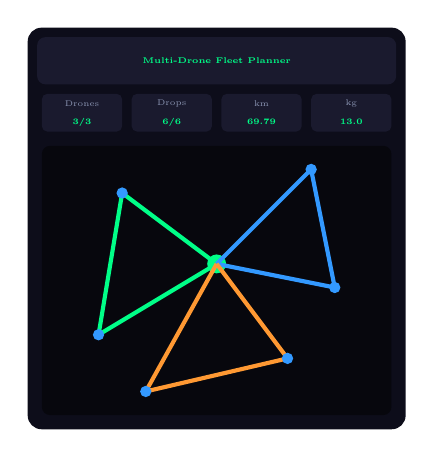
\begin{tikzpicture}[scale=0.6, transform shape]
    % Dashboard mockup
    \fill[darkbg, rounded corners=5pt] (0,0) rectangle (8,8.5);
    
    % Header
    \fill[cardbg, rounded corners=3pt] (0.2,7.3) rectangle (7.8,8.3);
    \node[font=\tiny\bfseries, text=neongreen] at (4,7.8) {Multi-Drone Fleet Planner};
    
    % Metrics
    \foreach \i/\val/\lab in {0/3\slash 3/Drones, 1/6\slash 6/Drops, 2/69.79/km, 3/13.0/kg} {
        \pgfmathsetmacro\xpos{0.3 + \i*1.9}
        \fill[cardbg, rounded corners=2pt] (\xpos,6.3) rectangle ++(1.7,0.8);
        \node[font=\tiny, text=softgray] at (\xpos+0.85,6.9) {\lab};
        \node[font=\tiny\bfseries, text=neongreen] at (\xpos+0.85,6.5) {\val};
    }
    
    % Map
    \fill[darkbg!50!black, rounded corners=3pt] (0.3,0.3) rectangle (7.7,6.0);
    
    % Warehouse
    \fill[neongreen] (4,3.5) circle (0.2);
    
    % Routes
    \draw[neongreen, line width=1.5pt] (4,3.5) -- (2,5) -- (1.5,2) -- (4,3.5);
    \draw[accentblue, line width=1.5pt] (4,3.5) -- (6,5.5) -- (6.5,3) -- (4,3.5);
    \draw[warnorange, line width=1.5pt] (4,3.5) -- (5.5,1.5) -- (2.5,0.8) -- (4,3.5);
    
    % Drop points
    \foreach \x/\y in {2/5, 1.5/2, 6/5.5, 6.5/3, 5.5/1.5, 2.5/0.8} {
        \fill[accentblue] (\x,\y) circle (0.12);
    }
\end{tikzpicture}
\end{column}
\end{columns}
\end{frame}

% ═══════════════════════════════════════
% SLIDE 18: FLEET RESULTS
% ═══════════════════════════════════════
\begin{frame}{Fleet Optimization Results}
\begin{center}
\textcolor{neongreen}{\textbf{Scenario: 1 Warehouse, 6 Drops, 3 Drones}}\\[0.3cm]
\end{center}

\begin{columns}[T]
\begin{column}{0.55\textwidth}
\small
\begin{tabular}{@{}lcccc@{}}
\toprule
\textcolor{neongreen}{\textbf{Drone}} & \textbf{Drops} & \textbf{Dist} & \textbf{Weight} & \textbf{Battery} \\
\midrule
\textcolor{neongreen}{D1} & D2, D5 & 22.31 km & 2.3 kg & 7.4\% \\
\textcolor{accentblue}{D2} & D1, D3, D6 & 28.14 km & 2.1 kg & 9.4\% \\
\textcolor{warnorange}{D3} & D4 & 19.34 km & 1.5 kg & 6.4\% \\
\midrule
\textbf{Total} & \textbf{6/6} & \textbf{69.79} & \textbf{5.9} & -- \\
\bottomrule
\end{tabular}

\vspace{0.4cm}
\begin{exampleblock}{Key Metrics}
\footnotesize
\begin{itemize}
    \item All 6 drops served $\checkmark$
    \item Max battery: 9.4\% (of 300 km range) $\checkmark$
    \item OR-Tools converged in $<$ 10s $\checkmark$
    \item All paths avoid Red zones $\checkmark$
\end{itemize}
\end{exampleblock}
\end{column}
\begin{column}{0.42\textwidth}
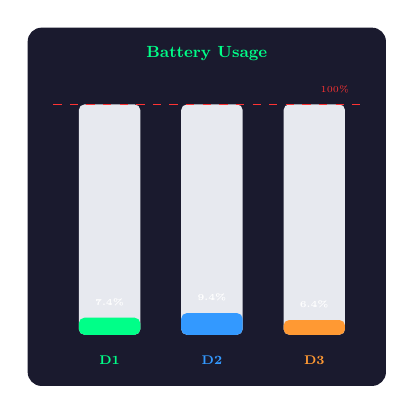
\begin{tikzpicture}[scale=0.65, transform shape]
    \fill[cardbg, rounded corners=5pt] (0,0) rectangle (7,7);
    \node[font=\small\bfseries, text=neongreen] at (3.5,6.5) {Battery Usage};
    
    % Battery bars
    \foreach \i/\pct/\col/\name in {0/7.4/neongreen/D1, 1/9.4/accentblue/D2, 2/6.4/warnorange/D3} {
        \pgfmathsetmacro\xpos{1.0 + \i*2.0}
        % Background bar
        \fill[softgray!20, rounded corners=2pt] (\xpos,1.0) rectangle ++(1.2,4.5);
        % Fill bar
        \pgfmathsetmacro\fillh{\pct/100*4.5}
        \fill[\col, rounded corners=2pt] (\xpos,1.0) rectangle ++(1.2,\fillh);
        % Label
        \node[font=\scriptsize\bfseries, text=\col] at (\xpos+0.6,0.5) {\name};
        \node[font=\tiny\bfseries, text=white] at (\xpos+0.6,1.0+\fillh+0.3) {\pct\%};
    }
    
    % 100% line
    \draw[dangerred, dashed] (0.5,5.5) -- (6.5,5.5);
    \node[font=\tiny, text=dangerred] at (6.0,5.8) {100\%};
\end{tikzpicture}
\end{column}
\end{columns}
\end{frame}

% ═══════════════════════════════════════
% SLIDE 19: PATHFINDING RESULTS
% ═══════════════════════════════════════
\begin{frame}{Pathfinding Performance Analysis}
\begin{columns}[T]
\begin{column}{0.50\textwidth}
\textcolor{neongreen}{\textbf{A* Pathfinding Speed:}}\\[0.2cm]
\small
\begin{tabular}{@{}lcccc@{}}
\toprule
\textbf{Mission} & \textbf{Direct} & \textbf{Safe} & \textbf{Detour} & \textbf{Time} \\
\midrule
N$\to$S & 8.12 & 9.47 & 1.17$\times$ & 47ms \\
E$\to$W & 5.63 & 6.21 & 1.10$\times$ & 32ms \\
Cross & 12.45 & 15.83 & 1.27$\times$ & 89ms \\
Dense & 3.21 & 4.56 & 1.42$\times$ & 28ms \\
\bottomrule
\end{tabular}

\vspace{0.3cm}
\begin{exampleblock}{Summary}
\footnotesize
\begin{itemize}
    \item Average detour: \textbf{1.24$\times$} (24\% extra)
    \item All paths computed in \textbf{$<$ 100ms}
    \item Zero Red zone violations
    \item Real-time interactive planning
\end{itemize}
\end{exampleblock}
\end{column}
\begin{column}{0.45\textwidth}
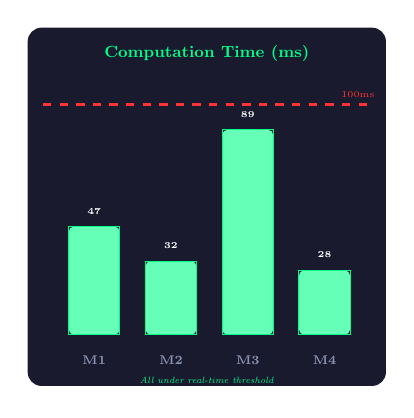
\begin{tikzpicture}[scale=0.65, transform shape]
    \fill[cardbg, rounded corners=5pt] (0,0) rectangle (7,7);
    \node[font=\small\bfseries, text=neongreen] at (3.5,6.5) {Computation Time (ms)};
    
    % Bar chart
    \foreach \i/\val/\name in {0/47/M1, 1/32/M2, 2/89/M3, 3/28/M4} {
        \pgfmathsetmacro\xpos{0.8 + \i*1.5}
        \pgfmathsetmacro\barh{\val/100*4.5}
        \fill[neongreen!60, rounded corners=2pt] (\xpos,1.0) rectangle ++(1.0,\barh);
        \draw[neongreen] (\xpos,1.0) rectangle ++(1.0,\barh);
        \node[font=\tiny\bfseries, text=white] at (\xpos+0.5,1.0+\barh+0.3) {\val};
        \node[font=\scriptsize\bfseries, text=softgray] at (\xpos+0.5,0.5) {\name};
    }
    
    % 100ms threshold
    \draw[dangerred, dashed, thick] (0.3,1.0+4.5) -- (6.7,1.0+4.5);
    \node[font=\tiny, text=dangerred, anchor=east] at (6.9,5.7) {100ms};
    
    \node[font=\tiny\itshape, text=neongreen] at (3.5,0.1) {All under real-time threshold};
\end{tikzpicture}
\end{column}
\end{columns}
\end{frame}

% ═══════════════════════════════════════
% SLIDE 20: COMPARISON
% ═══════════════════════════════════════
\begin{frame}{Algorithm Comparison}
\begin{center}
\small
\begin{tabular}{@{}p{2.5cm}ccccc@{}}
\toprule
\textcolor{neongreen}{\textbf{Algorithm}} & \textbf{Optimal?} & \textbf{Complete?} & \textbf{Speed} & \textbf{Smooth?} & \textbf{Grid?} \\
\midrule
\rowcolor{neongreen!10}
\textbf{A* + String} & \textcolor{neongreen}{\checkmark} & \textcolor{neongreen}{\checkmark} & Fast & \textcolor{neongreen}{\checkmark} & Yes \\
Dijkstra & \textcolor{neongreen}{\checkmark} & \textcolor{neongreen}{\checkmark} & 3--5$\times$ slower & \textcolor{dangerred}{$\times$} & Yes \\
RRT* & Asymptotic & Probabilistic & Variable & \textcolor{dangerred}{$\times$} & No \\
Theta* & \textcolor{neongreen}{\checkmark} & \textcolor{neongreen}{\checkmark} & Similar & \textcolor{neongreen}{\checkmark} & Yes \\
Potential Field & \textcolor{dangerred}{$\times$} & \textcolor{dangerred}{$\times$} & Very fast & \textcolor{neongreen}{\checkmark} & No \\
\bottomrule
\end{tabular}
\end{center}

\vspace{0.3cm}
\begin{columns}[T]
\begin{column}{0.48\textwidth}
\begin{exampleblock}{Why A* + String-Pulling?}
\footnotesize
\begin{itemize}
    \item Guarantees optimal + complete
    \item String-pulling gives smooth paths
    \item Simple implementation on grids
    \item Predictable, deterministic results
\end{itemize}
\end{exampleblock}
\end{column}
\begin{column}{0.48\textwidth}
\begin{alertblock}{Limitations}
\footnotesize
\begin{itemize}
    \item Grid resolution limits precision
    \item Static environment only
    \item 2D planning (constant altitude)
    \item No wind/weather modeling
\end{itemize}
\end{alertblock}
\end{column}
\end{columns}
\end{frame}

% ═══════════════════════════════════════
% SLIDE 21: DEPLOYMENT
% ═══════════════════════════════════════
\begin{frame}{Deployment on Hugging Face Spaces}
\begin{columns}[T]
\begin{column}{0.55\textwidth}
\textcolor{neongreen}{\textbf{Live Public Application}}\\[0.2cm]
\small
\begin{itemize}
    \item[\textcolor{neongreen}{$\bullet$}] Hosted on \textbf{Hugging Face Spaces} (free tier)
    \item[\textcolor{neongreen}{$\bullet$}] Streamlit SDK, containerized deployment
    \item[\textcolor{neongreen}{$\bullet$}] \textbf{No installation required} -- browser only
    \item[\textcolor{neongreen}{$\bullet$}] Dual-mode: Single Drone + Fleet
\end{itemize}

\vspace{0.3cm}
\textcolor{accentblue}{\textbf{Access URL:}}\\[0.1cm]
{\small\url{https://huggingface.co/spaces/harphool17/drone-route-planner}}

\vspace{0.3cm}
\textcolor{warnorange}{\textbf{Deployment Stack:}}
\begin{itemize}\small
    \item \texttt{app.py} $\rightarrow$ unified entry point
    \item \texttt{requirements.txt} $\rightarrow$ auto-install
    \item \texttt{data/} + \texttt{output/} $\rightarrow$ pre-computed maps
    \item Git push $\rightarrow$ auto-build \& deploy
\end{itemize}
\end{column}
\begin{column}{0.42\textwidth}
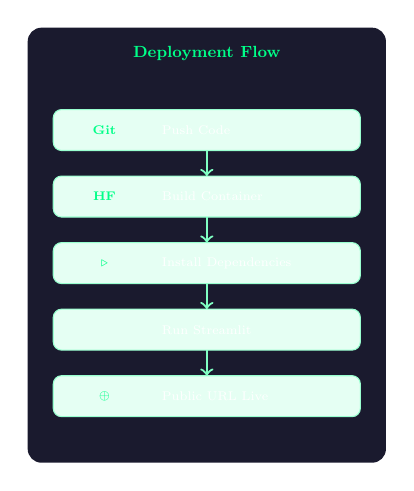
\begin{tikzpicture}[scale=0.65, transform shape]
    % Deployment flow
    \fill[cardbg, rounded corners=5pt] (0,0) rectangle (7,8.5);
    \node[font=\small\bfseries, text=neongreen] at (3.5,8.0) {Deployment Flow};
    
    % Steps
    \foreach \i/\icon/\text in {
        0/{Git}/Push Code,
        1/{HF}/Build Container,
        2/{$\triangleright$}/Install Dependencies,
        3/{$\checkmark$}/Run Streamlit,
        4/{$\oplus$}/Public URL Live
    } {
        \pgfmathsetmacro\ypos{6.5 - \i*1.3}
        \fill[neongreen!10, rounded corners=3pt] (0.5,\ypos-0.4) rectangle (6.5,\ypos+0.4);
        \draw[neongreen!40, rounded corners=3pt] (0.5,\ypos-0.4) rectangle (6.5,\ypos+0.4);
        \node[font=\scriptsize\bfseries, text=neongreen] at (1.5,\ypos) {\icon};
        \node[font=\scriptsize, text=white, anchor=west] at (2.5,\ypos) {\text};
    }
    
    % Arrows between steps
    \foreach \i in {0,...,3} {
        \pgfmathsetmacro\ya{6.5 - \i*1.3 - 0.4}
        \pgfmathsetmacro\yb{6.5 - (\i+1)*1.3 + 0.4}
        \draw[neongreen!50, ->, thick] (3.5,\ya) -- (3.5,\yb);
    }
\end{tikzpicture}
\end{column}
\end{columns}
\end{frame}

% ═══════════════════════════════════════
% SLIDE 22: FUTURE WORK
% ═══════════════════════════════════════
\begin{frame}{Future Work}
\begin{columns}[T]
\begin{column}{0.48\textwidth}
\begin{block}{Short-Term}
\begin{itemize}\small
    \item[\textcolor{neongreen}{1.}] \textbf{Dynamic Obstacles}\\ADS-B data for moving drones/aircraft
    \item[\textcolor{neongreen}{2.}] \textbf{Weather Integration}\\Wind speed $\rightarrow$ battery adjustment
    \item[\textcolor{neongreen}{3.}] \textbf{3D Path Planning}\\Altitude-varying paths with layered grids
\end{itemize}
\end{block}
\end{column}
\begin{column}{0.48\textwidth}
\begin{block}{Long-Term}
\begin{itemize}\small
    \item[\textcolor{accentblue}{4.}] \textbf{Multi-Depot VRP}\\Multiple warehouses
    \item[\textcolor{accentblue}{5.}] \textbf{NVIDIA cuOpt}\\GPU-accelerated VRP for 500+ drops
    \item[\textcolor{accentblue}{6.}] \textbf{ML Heuristics}\\Neural network-trained A* heuristic
\end{itemize}
\end{block}
\end{column}
\end{columns}
\end{frame}

% ═══════════════════════════════════════
% SLIDE 23: CONCLUSION
% ═══════════════════════════════════════
\begin{frame}{Conclusion}
\begin{center}
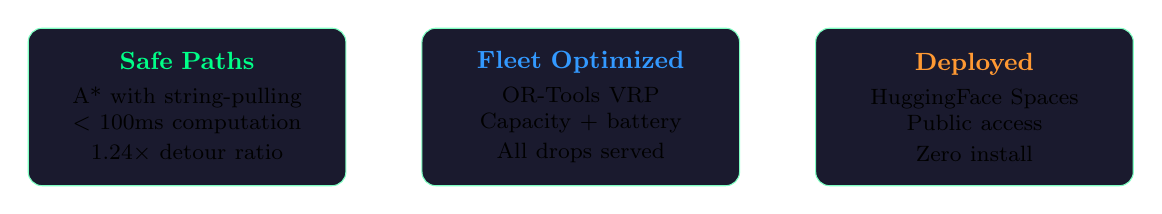
\begin{tikzpicture}[
    cbox/.style={rectangle, draw=neongreen!50, fill=cardbg, text width=3.8cm, text centered, rounded corners=5pt, minimum height=2.0cm, font=\small},
]
    \node[cbox] (c1) at (0,0) {\textcolor{neongreen}{\textbf{Safe Paths}}\\[0.1cm]\footnotesize A* with string-pulling\\$<$ 100ms computation\\1.24$\times$ detour ratio};
    
    \node[cbox] (c2) at (5,0) {\textcolor{accentblue}{\textbf{Fleet Optimized}}\\[0.1cm]\footnotesize OR-Tools VRP\\Capacity + battery\\All drops served};
    
    \node[cbox] (c3) at (10,0) {\textcolor{warnorange}{\textbf{Deployed}}\\[0.1cm]\footnotesize HuggingFace Spaces\\Public access\\Zero install};
\end{tikzpicture}
\end{center}

\vspace{0.5cm}
\begin{exampleblock}{Summary}
\small
Built a \textbf{complete, deployable} drone delivery system specific to \textbf{Indian regulations}, integrating A* pathfinding, OR-Tools fleet optimization, and interactive visualization -- accessible to anyone via a public URL.
\end{exampleblock}
\end{frame}

% ═══════════════════════════════════════
% SLIDE 24: REFERENCES
% ═══════════════════════════════════════
\begin{frame}{References}
\footnotesize
\begin{enumerate}[leftmargin=*]
    \item Hart, P.E., Nilsson, N.J., Raphael, B. ``A formal basis for heuristic determination of minimum cost paths.'' \textit{IEEE Trans. SSC.}, 1968.
    \item Dijkstra, E.W. ``A note on two problems in connexion with graphs.'' \textit{Numerische Mathematik}, 1959.
    \item Karaman, S., Frazzoli, E. ``Sampling-based algorithms for optimal motion planning.'' \textit{IJRR}, 2011.
    \item Harabor, D., Grastien, A. ``Online graph pruning for pathfinding on grid maps.'' \textit{AAAI}, 2011.
    \item Dantzig, G.B., Ramser, J.H. ``The truck dispatching problem.'' \textit{Management Science}, 1959.
    \item Murray, C.C., Chu, A.G. ``The flying sidekick TSP.'' \textit{Transportation Research Part C}, 2015.
    \item DGCA, ``The Drone Rules, 2021.'' Ministry of Civil Aviation, India.
    \item Google, ``OR-Tools: Optimization tools.'' developers.google.com/optimization, 2023.
    \item Khatib, O. ``Real-time obstacle avoidance for manipulators.'' \textit{IJRR}, 1986.
\end{enumerate}
\end{frame}

% ═══════════════════════════════════════
% SLIDE 25: THANK YOU
% ═══════════════════════════════════════
\begin{frame}[plain]
\begin{tikzpicture}[remember picture, overlay]
    \fill[top color=darkbg, bottom color=cardbg] (current page.north west) rectangle (current page.south east);
    \draw[neongreen!30, line width=0.5pt] ([yshift=-2cm]current page.north west) -- ([yshift=-2cm]current page.north east);
    \draw[neongreen!30, line width=0.5pt] ([yshift=2cm]current page.south west) -- ([yshift=2cm]current page.south east);
\end{tikzpicture}
\begin{center}
\vspace{2cm}
{\fontsize{36}{40}\selectfont\textcolor{neongreen}{\textbf{Thank You!}}}\\[0.8cm]
{\large\textcolor{white}{Questions \& Discussion}}\\[1.0cm]
{\small\textcolor{softgray}{Live Demo:}}\\[0.2cm]
{\small\textcolor{accentblue}{\url{https://huggingface.co/spaces/harphool17/drone-route-planner}}}\\[0.8cm]
{\footnotesize\textcolor{softgray}{Dr.\ Vipul Sharma $\cdot$ Aditya Acharya $\cdot$ Harphool Singh $\cdot$ Pradeep Kumar $\cdot$ Vishvendra}}\\[0.1cm]
{\footnotesize\textcolor{softgray}{Gati Shakti Vishwavidyalaya, Vadodara}}
\end{center}
\end{frame}

\end{document}
